\documentclass[border=5pt]{standalone}
\usepackage{amssymb}
\usepackage{tikz}
\usetikzlibrary{positioning, arrows.meta, patterns, calc}
\begin{document}
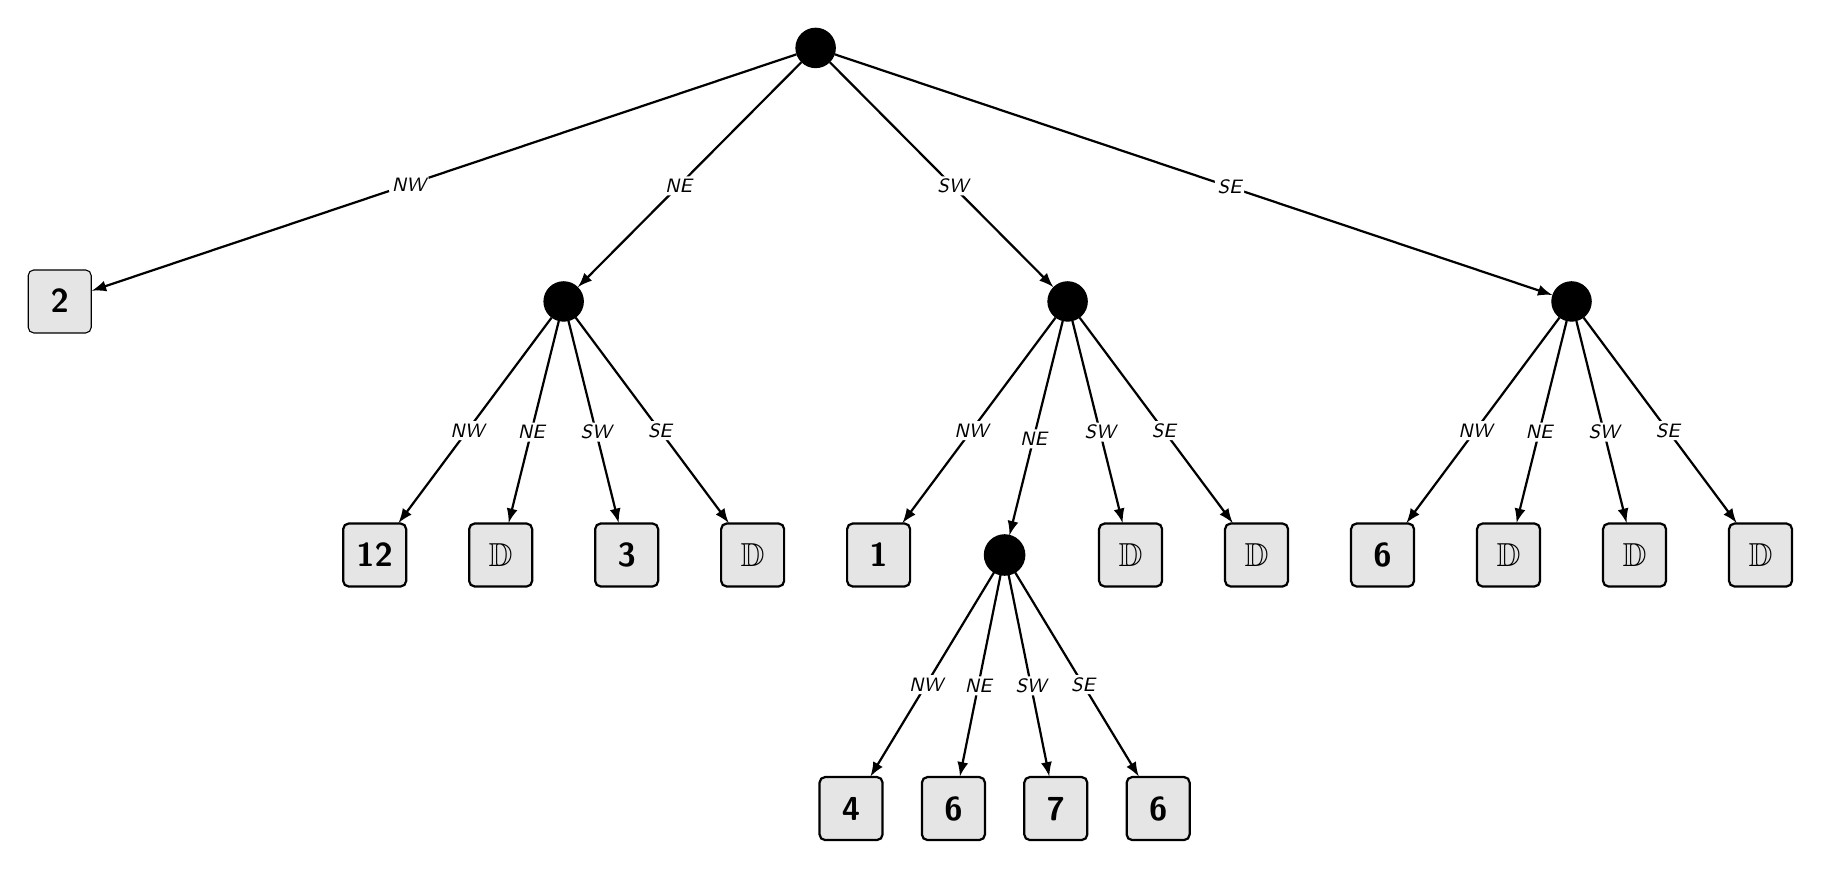
\begin{tikzpicture}[
    grow=down,
    font=\sffamily,
    level 1/.style={sibling distance=6.4cm, level distance=3.22cm},
    level 2/.style={sibling distance=1.6cm, level distance=3.22cm},
    level 3/.style={sibling distance=1.3cm, level distance=3.22cm},
    edge from parent/.style={draw, -latex, thick},
    int/.style={draw, circle, fill=black, minimum size=0.5cm, inner sep=0pt},
    leaf/.style={draw, rectangle, fill=gray!20, font=\sffamily\large\bfseries,
                 minimum size=0.8cm, inner sep=2pt, rounded corners=2pt},
    q/.style={font=\sffamily\scriptsize\itshape, pos=0.55, fill=white,
              inner sep=1pt, rounded corners=1pt},
  ]

\node[int] { }
    child { node[leaf] {2} edge from parent node[q] {NW} }
    child {
        node[int] { }
        child { node[leaf] {12} edge from parent node[q] {NW} }
        child { node[leaf] {$\mathbb{D}$} edge from parent node[q] {NE} }
        child { node[leaf] {3} edge from parent node[q] {SW} }
        child { node[leaf] {$\mathbb{D}$} edge from parent node[q] {SE} }
        edge from parent node[q] {NE}
    }
    child {
        node[int] { }
        child { node[leaf] {1} edge from parent node[q] {NW} }
        child { node[int] { }
            child { node[leaf] {4} edge from parent node[q] {NW} }
            child { node[leaf] {6} edge from parent node[q] {NE} }
            child { node[leaf] {7} edge from parent node[q] {SW} }
            child { node[leaf] {6} edge from parent node[q] {SE} }
            edge from parent node[q] {NE}
        }
        child { node[leaf] {$\mathbb{D}$} edge from parent node[q] {SW} }
        child { node[leaf] {$\mathbb{D}$} edge from parent node[q] {SE} }
        edge from parent node[q] {SW}
    }
    child {
        node[int] { }
        child { node[leaf] {6} edge from parent node[q] {NW} }
        child { node[leaf] {$\mathbb{D}$} edge from parent node[q] {NE} }
        child { node[leaf] {$\mathbb{D}$} edge from parent node[q] {SW} }
        child { node[leaf] {$\mathbb{D}$} edge from parent node[q] {SE} }
        edge from parent node[q] {SE}
    };
\end{tikzpicture}
\end{document}
